\documentclass[tikz,border=2pt]{standalone}
\usepackage{amsmath}
\usepackage{pgfplots}
\pgfplotsset{compat=1.18}
\usetikzlibrary{arrows.meta}
\begin{document}
% Example 1 game, player 2's expected payoffs against the belief pi_2(T)=x: L gives 3-2x, M gives 1+x,
% R gives 0. The upper envelope is the best response: L for x<2/3, M for x>2/3; at x=0.4, L (2.2>1.4).
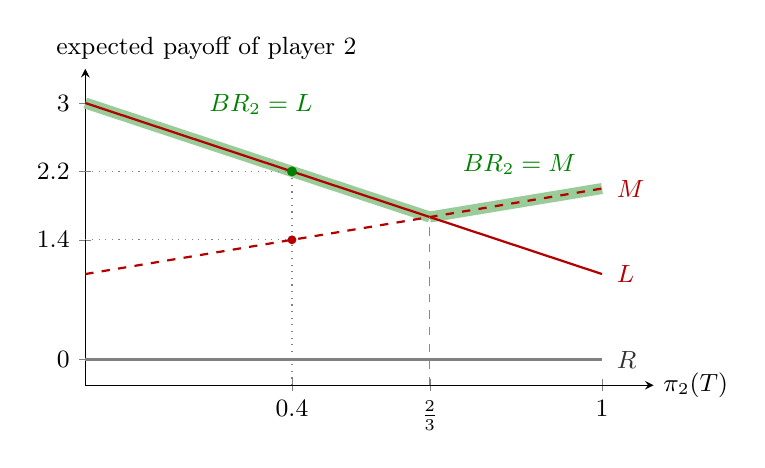
\begin{tikzpicture}[font=\small, >={Latex[length=2mm]}]
  \begin{axis}[
    axis lines=left,
    xmin=0, xmax=1.1, ymin=-0.3, ymax=3.4,
    xtick={0.4,0.6667,1}, xticklabels={$0.4$,$\tfrac23$,$1$},
    ytick={0,1.4,2.2,3}, yticklabels={$0$,$1.4$,$2.2$,$3$},
    xlabel={$\pi_2(T)$}, ylabel={expected payoff of player 2},
    xlabel style={at={(axis description cs:1,0)}, anchor=west},
    ylabel style={at={(axis description cs:0,1)}, anchor=south west, rotate=-90, xshift=-14pt},
    tick label style={font=\small},
    samples=2, clip=false,
    width=8.8cm, height=5.6cm]
    % best response = upper envelope
    \addplot[green!50!black!40, line width=4pt, domain=0:0.6667] {3-2*x};
    \addplot[green!50!black!40, line width=4pt, domain=0.6667:1] {1+x};
    \addplot[red!70!black, thick, domain=0:1] {3-2*x};
    \addplot[red!70!black, thick, dashed, domain=0:1] {1+x};
    \addplot[gray, thick, domain=0:1] {0};
    \node[red!70!black, anchor=west] at (axis cs:1.01,1) {$L$};
    \node[red!70!black, anchor=west] at (axis cs:1.01,2) {$M$};
    \node[gray!40!black, anchor=west] at (axis cs:1.01,0) {$R$};
    % threshold and belief 0.4
    \draw[orange!90!black, dashed, thin] (axis cs:0.6667,-0.3) -- (axis cs:0.6667,1.6667);
    \draw[gray, thin, dotted] (axis cs:0.4,-0.3) -- (axis cs:0.4,2.2);
    \draw[gray, thin, dotted] (axis cs:0,2.2) -- (axis cs:0.4,2.2);
    \draw[gray, thin, dotted] (axis cs:0,1.4) -- (axis cs:0.4,1.4);
    \fill[green!50!black] (axis cs:0.4,2.2) circle (1.8pt);
    \fill[red!70!black] (axis cs:0.4,1.4) circle (1.6pt);
    \node[green!50!black, anchor=south] at (axis cs:0.34,2.75) {$BR_2=L$};
    \node[green!50!black, anchor=south] at (axis cs:0.84,2.05) {$BR_2=M$};
  \end{axis}
\end{tikzpicture}
\end{document}
